%%%%%%%%%%%%%%%%%%%%%%%%%%%%%%%%%%%%%%%%%%%%%%%%%%%%%%%%%%%%%%%%%
% Qualificacao de Doutorado / Dept Fisica, CFM, UFSC            %
% Eduardo@UFSC - 2015                                           %
%%%%%%%%%%%%%%%%%%%%%%%%%%%%%%%%%%%%%%%%%%%%%%%%%%%%%%%%%%%%%%%%%


%:::::::::::::::::::::::::::::::::::::::::::::::::::::::::::::::%
%                                                               %
%                          Capítulo 5                           %
%                                                               %
%:::::::::::::::::::::::::::::::::::::::::::::::::::::::::::::::%

%***************************************************************%
%                                                               %
%                     Diferential extintion                     %
%                                                               %
%***************************************************************%

\chapter{Extinção diferencial}
\label{sec:difextin}

Nosso objetivo é conseguir estimar fração de gás para nossas galáxias do \CAL através da conversão
de poeira em gás explorando uma conversão do tipo da Eq. \ref{eq:dust2gas}. Para isso vamos tentar
entender melhor a diferença entre os coeficientes de extinção por poeira adotados, realizando um
procedimento parecido e fazendo algumas comparações com um estudo de nosso grupo de populações
estelares, que ainda está para ser públicado, sobre extinção diferencial em galáxias do \SDSS.
Este estudo sobre extinção diferencial nas galáxias do \SDSS é parte da tese de Marielli de Souza
Schlickmann.

%\section{Definindo nossas variáveis}
\section{Estudo empírico}
\label{sec:difextin:emp}

De maneira a explorar as diferenças entre os coeficientes de extinção, identificamos duas variáveis
que nos ajudarão nesse processo:
\begin{eqnarray}
	\mathcal{D}_\tau\ &\equiv&\ \tauVN - \tauVS \\
	\label{eq:difftau}
	\mathcal{R}_\tau\ &\equiv&\ \frac{\tauVN}{\tauVS} 
	\label{eq:ratiotau}
\end{eqnarray}

\subsection{Comparação direta entre os coeficientes}
\label{sec:difextin:emp:comparetauV}

Neste capítulo (e nos seguintes) me atenho a discussão à perfis radiais, voltado para zonas ou pra
valores integrados quando pertinente. Na Fig. \ref{fig:tauVhisto} vemos a comparação direta entre os
coeficientes, juntamente com os histogramas de $\Dtau$ e $\Rtau$. O primeiro painel mostra a
comparação entre os coeficientes como na Fig. \ref{fig:tauVsynvsnebMask} para perfis radiais. Os dois
histogramas são de $\Dtau$ e $\Rtau$. Os valores da mediana (média) de $\Dtau$ são 0.31 (0.32) e de
$\Rtau$, 2.06 (2.46) e ambos mostram claramente a existência de uma extinção diferencial. Esse
resultado aparece da mesma forma para zonas e para as galáxias integradas. No trabalho de Marielli
com as galáxias do \SDSS cabe lembrar que a síntese de populações estelares foi feita apenas para
espectros integrados e com diferentes base de populações estelares e IMF, e ainda sim encontramos
valores parecidos que evidenciam o mesmo fenômeno, e que serve de base para a discussão que vem a
seguir.

\begin{figure}
	\centering
	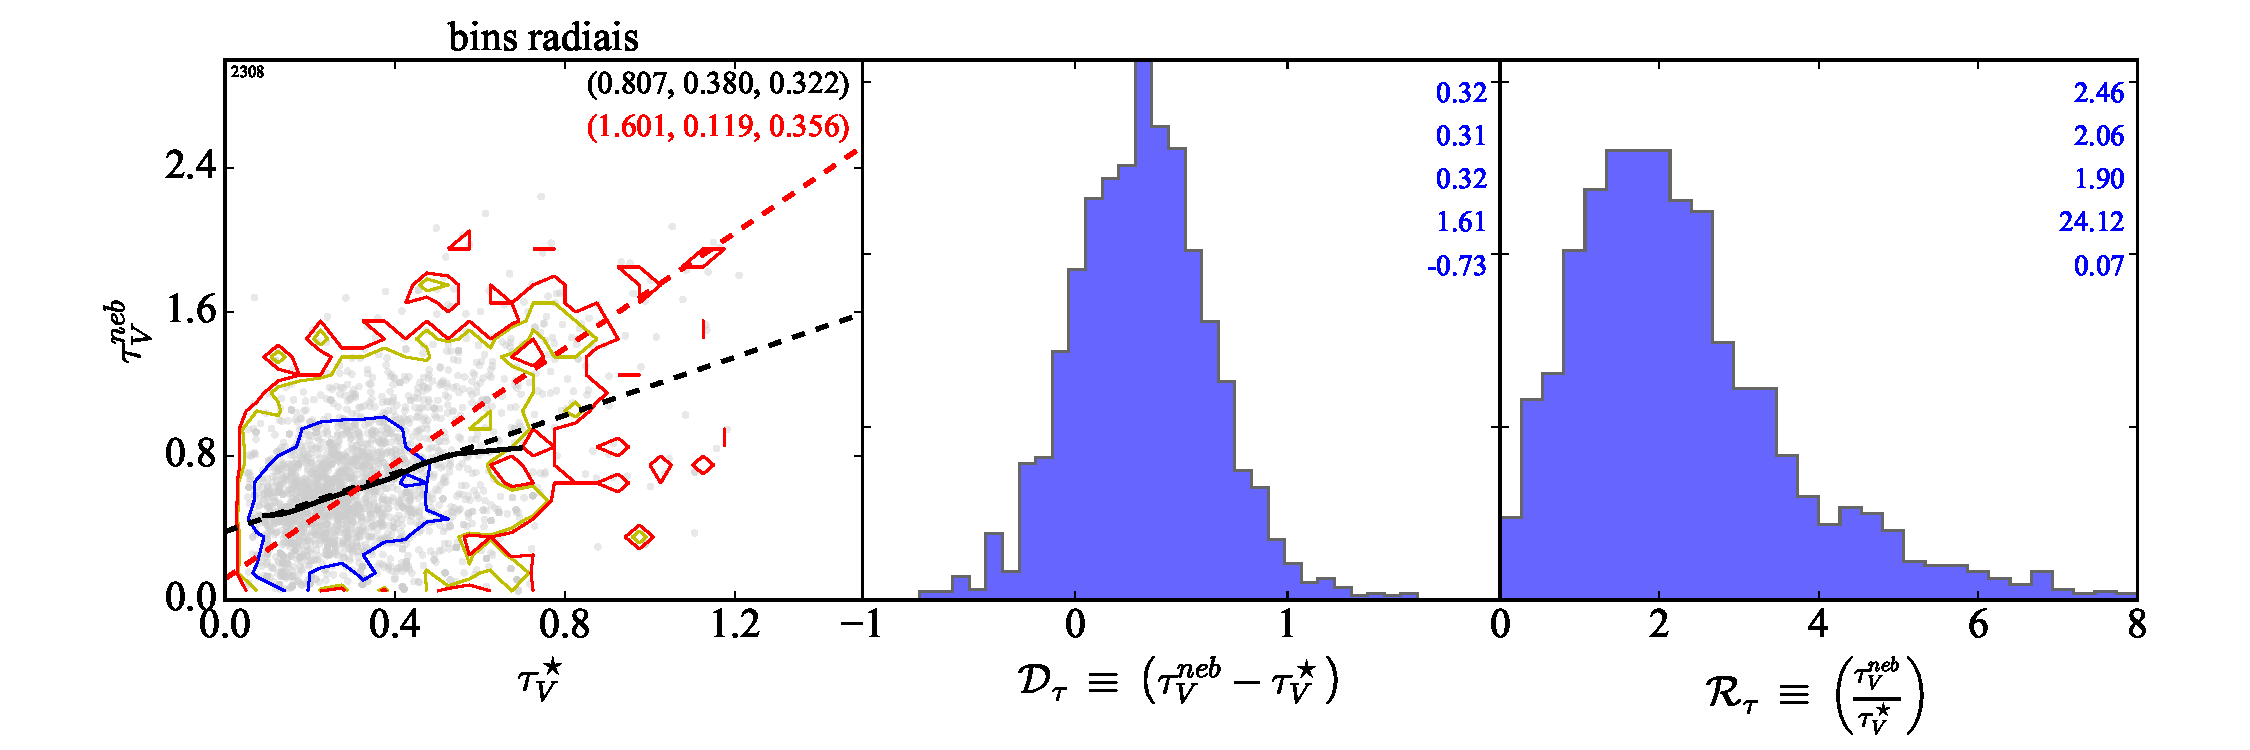
\includegraphics[width=0.99\textwidth]{figuras/histoTauVR.pdf}
	\caption[Comparação $\tauVS$ e histogramas de $\Dtau$ e $\Rtau$.]
	{\emph{Painel esquerdo}: Igual ao painel superior direito da Fig. \ref{fig:tauVsynvsnebMask}.
\emph{Painel central}: histograma normalizado de $\Dtau$. \emph{Painel esquerdo}: histograma
normalizado de $\Rtau$.}
	\label{fig:tauVhisto}
\end{figure}

\subsection{O papel de $x_Y$ e da $b/a$}
\label{sec:difextin:emp:xYcosi}

Pela relação entre os coeficientes vemos que há um espalhamento notável, entretanto, parece óbvio
que a extinção diferencial existe. Ao estudar todas as propriedades, galáxia por galáxia, vimos que
existe uma relação interessante entre $\Dtau$, $\Rtau$, a fração de populações jovens ($x_Y$) e
tambem a relação axial da galáxia ($b/a$). A primeira pela fato que relaciona regiões onde existam
populações mais jovens, ou seja, mais relacionadas a regiões formadoras de estrelas, ajudando-nos a quebrar um
pouco nessa ambiguidade nos valores de $\tauVS$ e a última pelo fato de afetar diretamente a forma
de modelar a extinção por poeira.

Para utilizar a relação axial vamos fazer uma pequena correção para a projeção do disco no plano do
céu:
\begin{equation}
	\varphi = \cos i = \left \{ \begin{matrix} \sqrt{\frac{(b/a)^2 - (0.13)^2}{1 - (0.13)^2}},
	&\mbox{se }b/a > 0.13 \\ 0.05, &\mbox{se }b/a <= 0.13 \end{matrix}\right
\end{equation}
\noindent onde $i$ é o ângulo de inclinação da galáxia e $0.13$ é o valor da relação
axial intrinseca de uma galáxia mais frontal possível ({\em edge-on}). Valores com $b/a$ <= 0.13
recebem o valor da menor inclinação de nossa amostra (0.05) ao invés de 0 para não haver problemas
matemáticos futuros. Esse é um refinamento que altera levemente o valor de $b/a$ e praticamente só
afeta as galáxias com $b/a$ < 0.4.

\begin{figure}
	\centering
	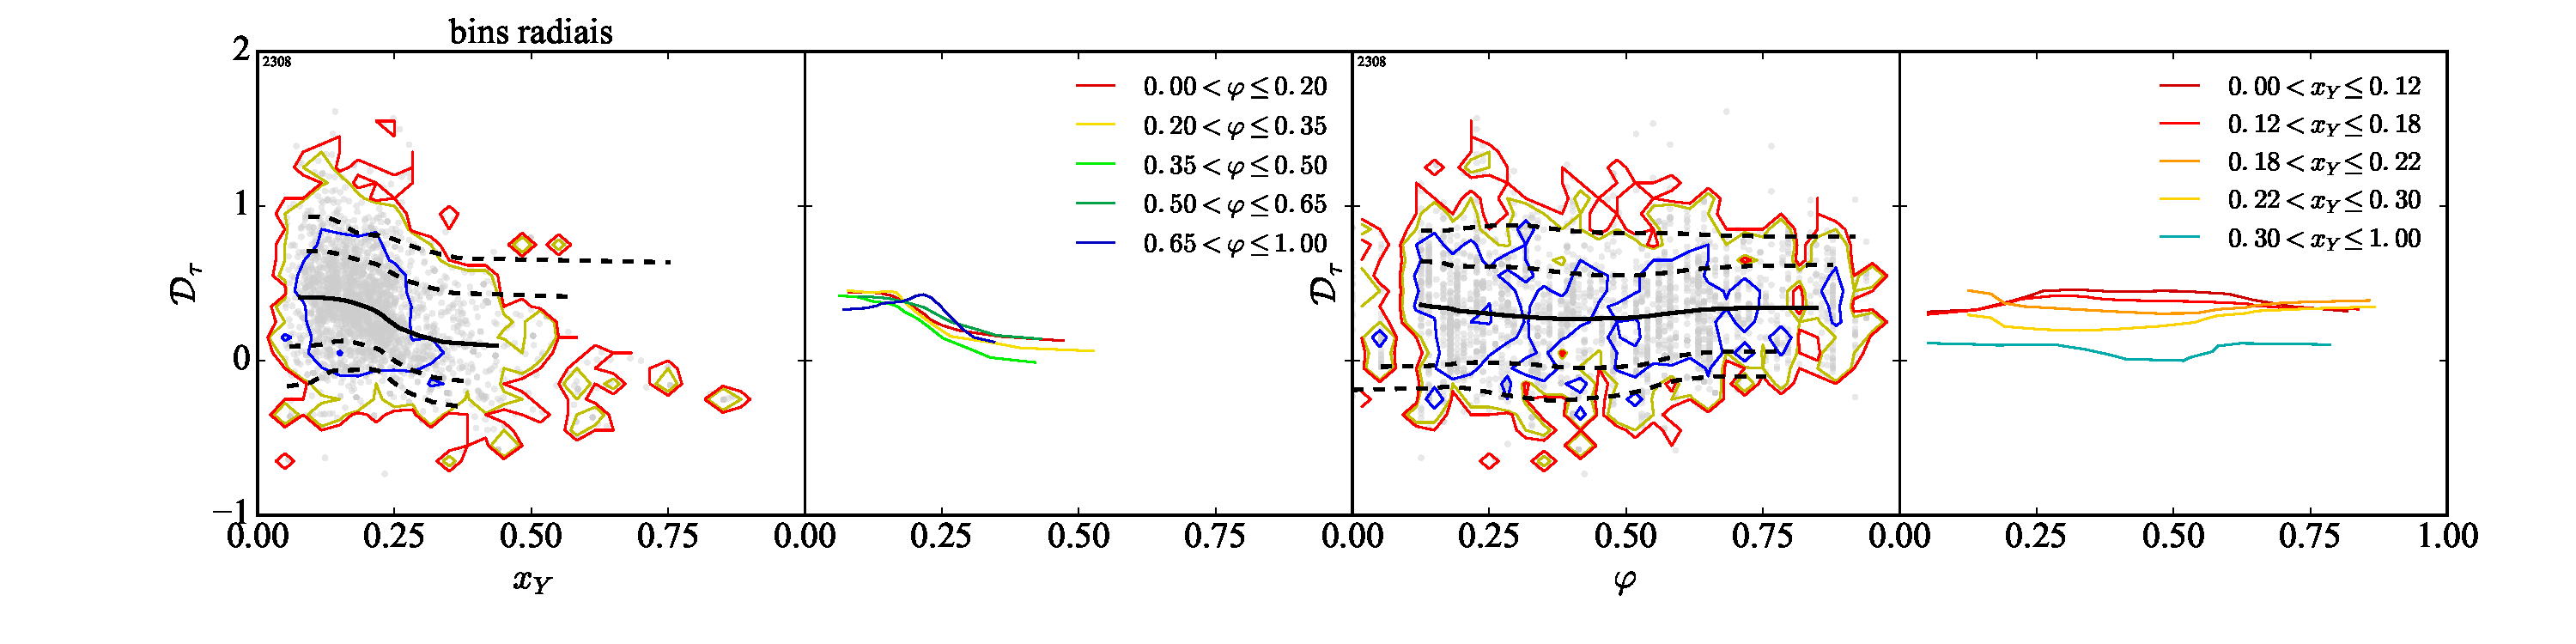
\includegraphics[width=0.99\textwidth]{figuras/DtauR.pdf}
	\caption[$\Dtau$, $x_Y$ e $\varphi$.]
	{\emph{Primeiro painel}: $\Dtau$ versus $x_Y$ para nossa amostra. Os contornos definem
$1\sigma$, $2\sigma$ e $3\sigma$ da distribuição. As linhas marcam a mediana (linha contínua) e os
5,16,64,95 percentis (linhas tracejadas). \emph{Segundo painel}: as medianas da mesma distribuição
quando dividimos nossa amostra em classes de $\varphi$. Os intervalos são criados para que contenham
praticamente o mesmo número de pontos. \emph{Terceiro painel}: igual ao primeiro mas versos
$\varphi$. \emph{Quarto painel}: igual a segundo mas com a amostra dividida em classes de $x_Y$.}
	\label{fig:Dtau}
\end{figure}

\begin{figure}
	\centering
	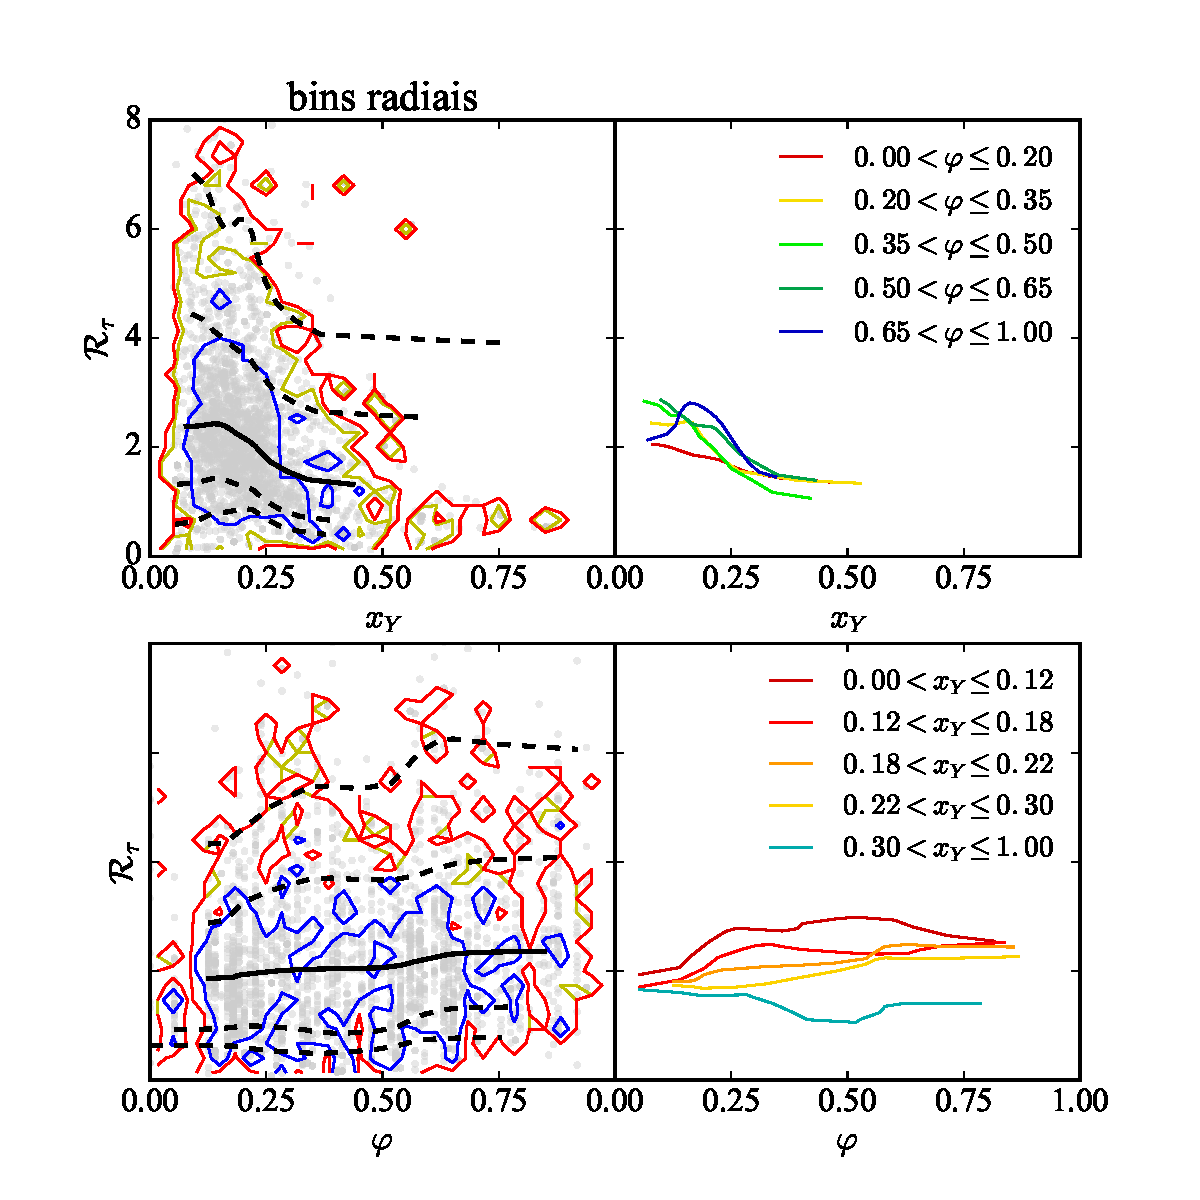
\includegraphics[width=0.99\textwidth]{figuras/RtauR.pdf}
	\caption[$\Rtau$, $x_Y$ e $\varphi$.]
	{Igual a Fig. \ref{fig:Dtau} mas com $\Rtau$.}
	\label{fig:Rtau}
\end{figure}

Na Fig. \ref{fig:Dtau} vemos como $\Dtau$ se relaciona com $\varphi$ e $x_Y$. No primeiro e
terceiro paineís vemos as distribuições, e no segundo e no quarto vemos as medianas para diferentes
classes da variável cruzada, isto é, distribuição contra $x_Y$ com os pontos divididos em classes de
$\varphi$ e distribuição contra $\varphi$ em classes de $x_Y$. É clara a tendência de $\Dtau\ \to\
0$ quando $x_Y \to 1$. Pelo primeiro painel vemos que apesar da existência de uma anticorrelação
entre $\Dtau$ e $x_Y$, existe um espalhamento considerável. No segundo painel dividimos nossa
amostra em classes de $\varphi$ e parece não haver dependência. No terceiro e quarto painel
exploramos a relação $\Dtau$ e $\varphi$. $\Dtau$ não parece haver dependência com $\varphi$ mas
quando dividimos a amostra em classes de $x_y$ vemos que se confirma a anticorrelação.

Repetimos esse mesmo experimento para $\Rtau$ na Fig. \ref{fig:Rtau}. Observando a mediana parece
que $\Rtau \to 1$ quando $x_Y \to 1$, com uma $\Rtau \to 3 \sim 4$ quando $x_Y \to 0$. Vemos pelo
último painel que a anticorrelação com $x_Y$ segue, mas olhando o segundo painel vemos que parece
haver um pequeno afastamento entre as medianas da distribuição quando dividimos nessas classes de
$\varphi$, mas esse resultado não parece aparece muito quando olhamos o terceiro painel. Quando
fazemos o mesmo gráfico para as galáxias do \SDSS esse resultado é muito mais evidente, aparecendo
uma correlação entre $\Rtau$. Em primeira estância creio que isso se deve ao poder da estatística de
quase 1 milhão de pontos sendo 1 por galáxia. Nosso estudo para as galáxias integradas da nossa
amostra peca por estatística, pois temos apenas 184 pontos.

\section{Modelagem e interpretação}
\label{sec:difextin:modeleinterp}

Com esse cenário criado até agora neste capítulo, parece ser óbvio que $x_Y$ é fundamental em nossa
interpretação da extinção diferencial. O resultado da correlação entre $\Rtau$ e $\varphi$
não parece ser tão forte localmente quanto para valores integrados pois ele aparece muito melhor
quando olhamos para a amostra do \SDSS. Seguiremos aqui assumindo essa na linha de interpretação do
trabalho de extinção diferencial nas galáxias do \SDSS. Essa diferença esperamos discutir em um
futuro próximo e entra na lista de coisas para fazer, portando nesta seção vou apresentar o modelo
proposto na tese de Marielli e utilizar a mesma modelagem com nossos dados.

\subsection{O modelo}
\label{sec:difextin:modeleinterp:model}

Segundo tudo que vimos até agora, nosso modelo deve levar em conta que a luz proveniente das
populações jovens são atenuadas de maneira mais intensa que o meio interestelar. Além disso, deve
levar em conta que existe algum tipo de relação entre a razão entre os coeficientes seja afetada
diretamente pelo ângulo de inclinação da galáxia. Apesar de aqui estarmos utilizando $t_{SF} = 32$
milhões de anos, tanto na tese de Marielli quanto no artigo de \citet{Charlot.Fall.2000a} são
consideradas jovens todas as populações com idade menor que 10 milhões de anos. A interpretação da
influência de $\varphi$ foi relacionada a diferença entre geometria das regiões \Hii e a da galáxia.
As estrelas jovens, assim como as velhas, possuem atenuações semelhantes a do ISM dos discos
galáticos, mas as populações jovens possuem também a poeira de suas {\em birth-clouds}. Ou seja, se
modelarmos as regiões \Hii como esfericamente simétricas, o coeficiente de extinção não deve se
alterar quando mudamos a linha de visada entre o observador e a galáxia. Já para o ISM parece se
alterar bastante, portanto a razão entre os coeficientes deve se alterar no mesmo passo que a
inclinação se altera. Na Fig.
\ref{fig:model} fica melhor explicado.

\begin{figure}
	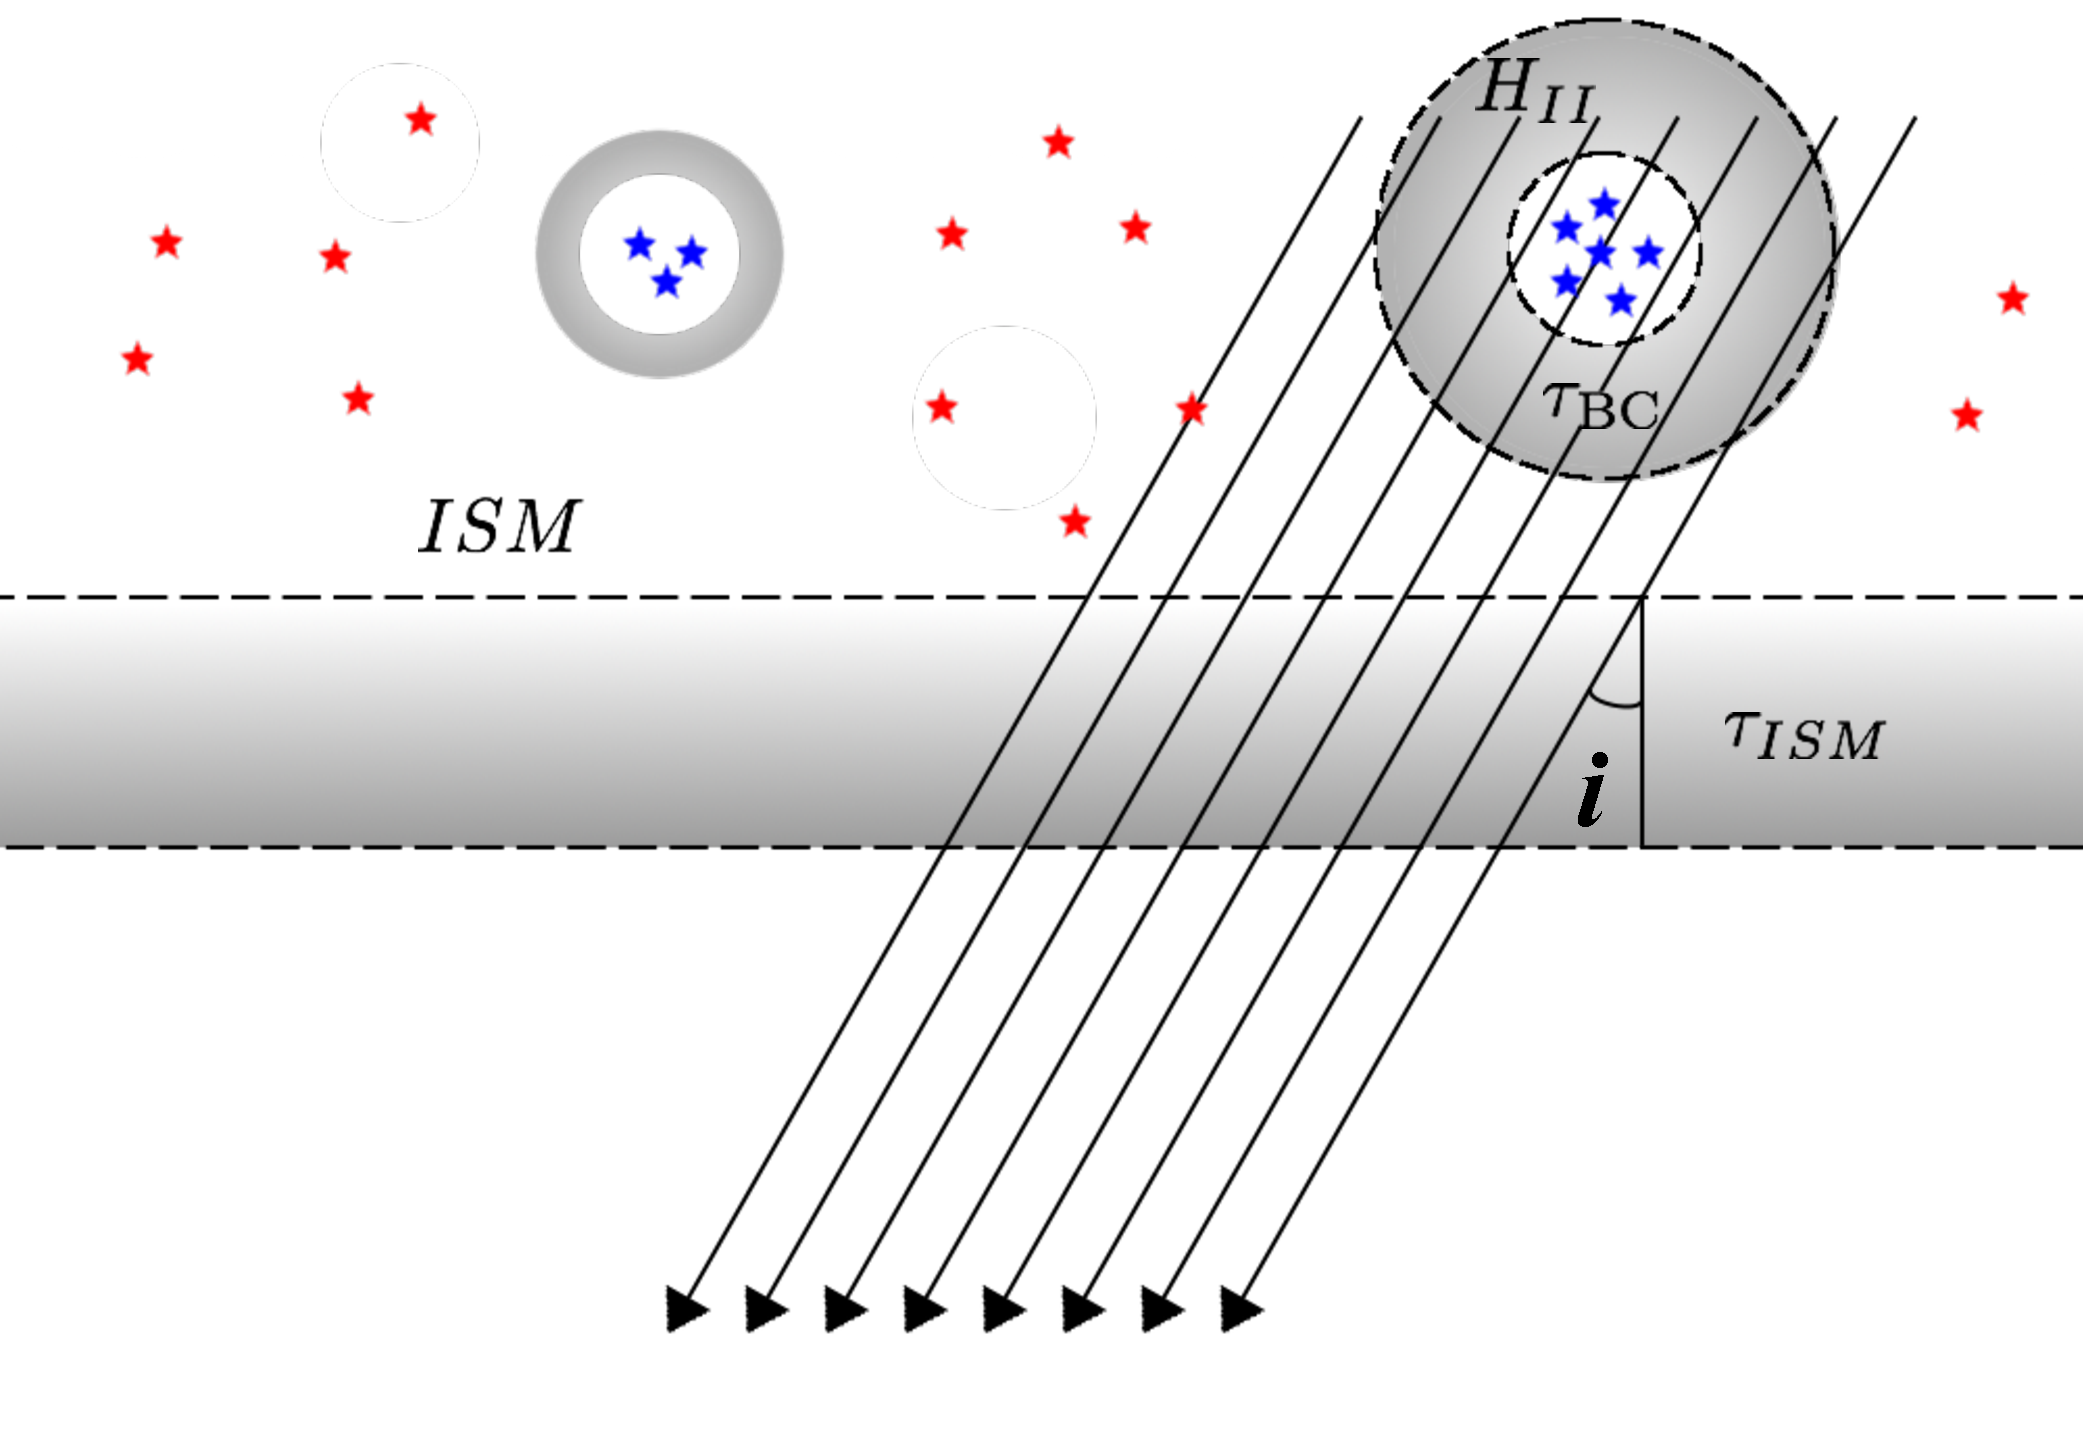
\includegraphics[width=0.99\textwidth]{figuras/Hiiregion_model.pdf}
	\caption[Modelo para extinção diferencial.]
	{}
	\label{fig:model}
\end{figure}

Essa figura juntamente com as considerações acima nos levam a a identificar um coeficiente de
extinção para as populações jovens e outro para as velhas da seguinte maneira:
\begin{eqnarray}
	\tau_O &=& \frac{\tau_{\mathrm{ISM}}}{\varphi} \\
	\label{eq:tauO}
	\tau_Y &=& \frac{\tau_{\mathrm{ISM}}}{\varphi} + \alpha\tau_{\mathrm{BC}}
	\label{eq:tauY} 
\end{eqnarray}
\noindent onde $\alpha$ entra para corrigir as possíveis diferenças entre a extinção para as
populações jovens e para as suas regiões \Hii associadas.

Para relacionar essas variávies com nossos observáveis, começamos identificando $\tau_Y$ como
$\tauVN$. Como comentamos na Sec. \ref{sec:synvsneb:tauv} $x_Y$ parece funcionar distribuindo os
pesos entre $\tau_O$ e $\tau_Y$ na interpretação de $\tauVS$, assim, podemos aproximar $\tauVS$
como:
\begin{equation}
	\tauVS \approx \tilde{\tau} \equiv x_Y \tau_Y + (1 - x_Y) \tau_O.
	\label{eq:tauVS}
\end{equation}
Com essa última equação fechamos nosso sistema e podemos escrever equações para $\tauISM$ e
$\tauBC$, além de trazer uma interpretação para o real significado de $\tauVS$. Trabalhando com as
Eqs. \ref{eq:tauO}, \ref{eq:tauY} e \ref{eq:tauVS} e identificando $\tau_Y = \tauVN$ obtemos:  
\begin{eqnarray}
	\tauBC &=& \frac{\tauVS - \tauVN}{1 - \alpha x_Y} \\
	\label{eq:tauBC}
	\tauISM &=& \varphi\frac{\tauVS - \alpha x_Y \tauVN}{1 - \alpha x_Y}  
	\label{eq:tauISM}
\end{eqnarray}

\section{Próximos passos}
\label{sec:difextin:nextsteps}

Ainda temos muito mais a fazer nessa direção. Ainda temos que comparar este modelo com os dados
para posteriormente podermos discutir as diferenças entre a aplicação deste modelo de extinção
diferencial para galáxias integradas e para perfis radiais (e consequentemente, para zonas também).

\subsection{Comparação com os dados.}
\label{sec:difextin:nextsteps:comp}

O primeiro passo no sentido da comparação deste modelo proposto com os dados é identificando as
nossas variáveis $\Dtau$ e $\Rtau$ no contexto da Fig. \ref{fig:model}:
\begin{eqnarray}
	\Dtau &=& (1 - \alpha x_Y) \tauBC \\
	\label{eq:DtauxY}
	\Rtau &=& \frac{\varphi^{-1} \tauISM + \alpha \tauBC}{\varphi^{-1} \tauISM + \alpha x_Y \tauBC}
\equiv \frac{1 + \alpha \varphi \rho}{1 + \alpha \varphi x_Y \rho}
	\label{eq:RtauxY}
\end{eqnarray}
\noindent onde $\rho = \frac{\tauBC}{\tauISM}$. 

Pelo histogram dessas variávis (Fig. \ref{fig:tauBCISM}) vemos que o cenário de extinção diferencial
persiste, com valores característicos (mediana) para $\tauBC$ de 0.39 e de $\tauISM$ 0.08. A razão
entre as medianas (médias) resulta em 4.9 (3.8). A mediana da razão nos leva a um valor um pouco
mais baixo, 3.43, mas há espalhamento muito grande nesta variável (devido aos valores de $\tauBC$ e
$\tauISM$ que passam por zero). 

\begin{figure}
	\centering
	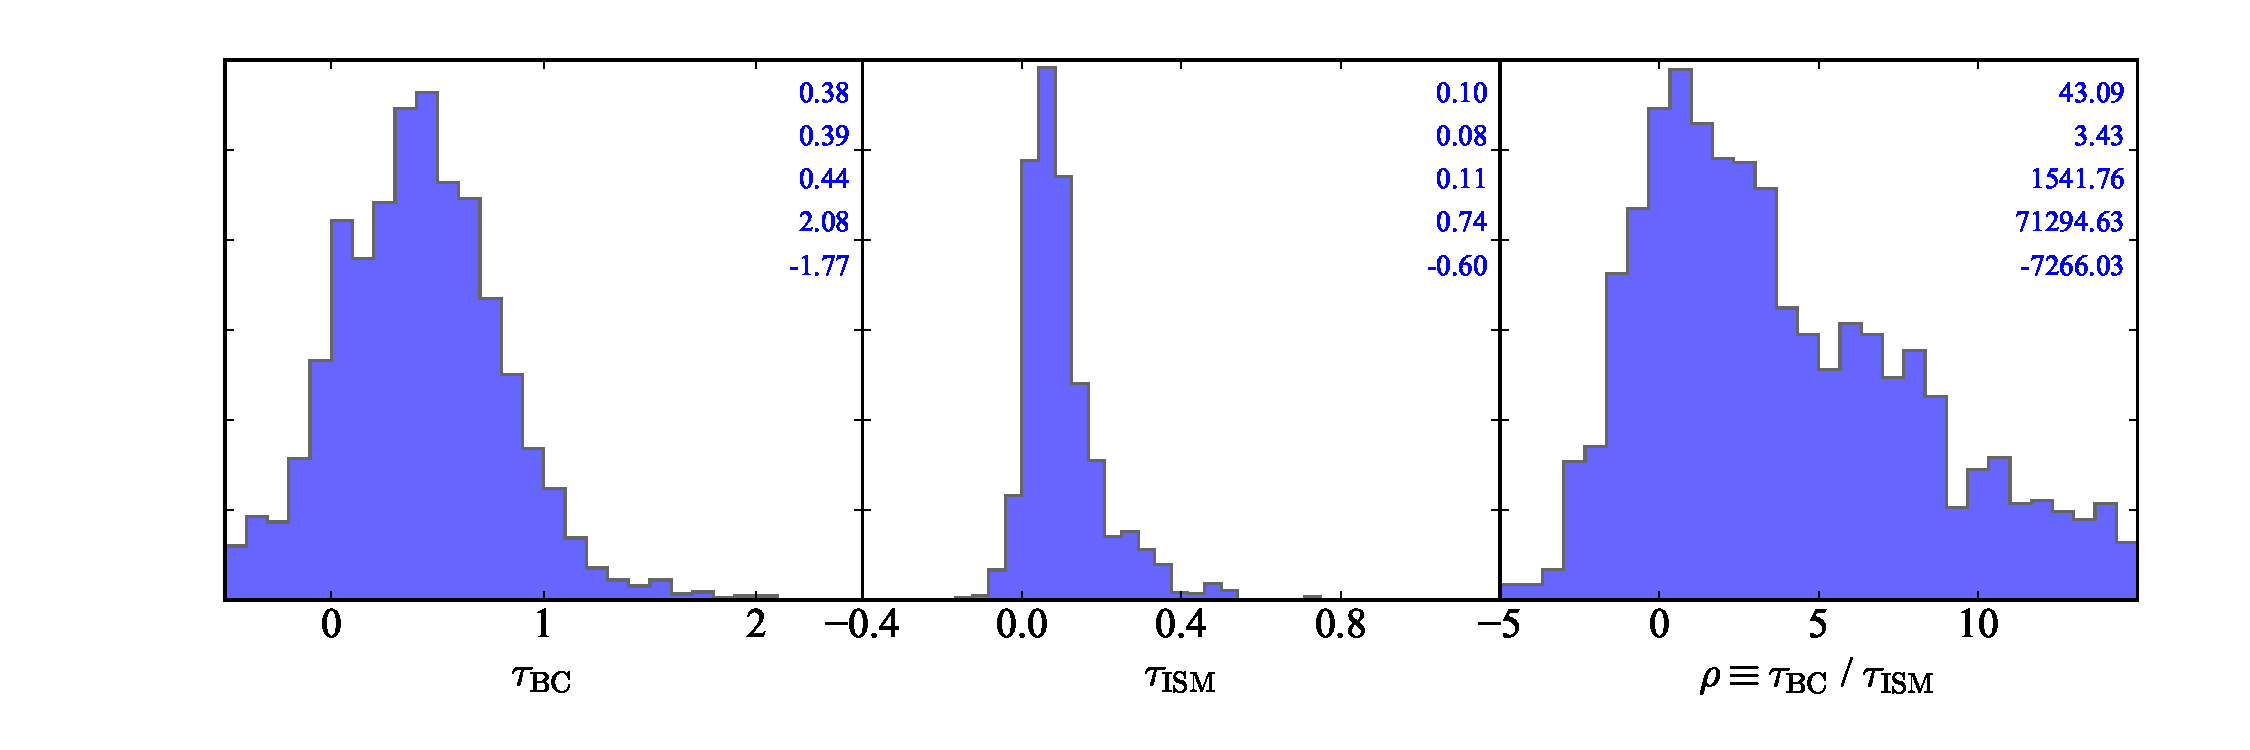
\includegraphics[width=0.99\textwidth]{figuras/tauISMBC_R.pdf}
	\caption[Histogramas de $\tauBC$, $\tauISM$ e $\rho$.]
	{Nos três painéis vemos os histogramas de $\tauBC$, $\tauISM$ e $\rho$. Os intervalos se estendem
para fora do gráfico, portanto, a última classe de cada histograma (em ambos os lados) contém todos
os pontos que ficaram para fora. Os valores nos cantos são os mesmos encontrados em todos os
histogramas deste trabalho: média, mediana, desvio padrão, máximo e mínimo.}
	\label{fig:tauBCISM}
\end{figure}

\subsection{Perfis radiais vs. propriedades integradas}
\label{sec:difextin:nextsteps:SDSSvsCALIFA}

Espectrografia de campo integrado está mudando a forma com que nós lidamos com os desafios atuais em
astrofísica. Os dados do \PCAL nos possibilitam calcular como as propriedades físicas se altera
dentro de uma galáxia. Ao estudar as populações estelares quando observamos uma região de uma
galáxia, ao invés de uma galáxia inteira, estamos olhando diferentes estágios de evolução química e
formação estelar, inclusive com uma diferença muito maior entre os coeficientes de extinção dentro
da mesma galáxia. As galáxias do \CAL estão dentro do mesmo intervalo de redshift de forma que todas
aproveitem o campo inteiro de observação, dessa forma, nossas zonas possuem diâmetros variando entre
200pc a 1kpc. Quando temos valores integrados, estamos olhando valores que representam uma galáxia
inteira (portanto uma ``soma'' de tudo o que acontece no bojo e no disco).  

%\subsubsection{$\Dtau}


% End of this chapter
